\section{Results}
\subsection{Performance}

The main reason to do image processing on the GPU and not on the traditional CPU was to gain better performance. Therefore, four tests are added to compare the different GPU environments against a non multithreaded CPU implementation. The four tests involve Linear Interpolation, Box Blur, Gaussian Blur and Separable Gaussian Blur. All blur algorithms have the same surrounding area of neighboring pixels. These algorithms can be found in Appendix A. The CPU code was executed on a machine with a Intel Xeon Processor(12M Cache, 2.80 GHz, 1600 MHz FSB) and the GPU kernels were executed on a NVIDIA GTX 760 card. The timings can be seen in Table \ref{tab}. In the GPU timings, the time it takes to copy input data to the GPU and output data to the CPU is included in the timings.

\begin {table}[H]
\caption {Performance timings} \label{tab} 
\begin{center}
    \begin{tabular}{| l | l | l | l | l |}
    \hline
    \textbf{Algorithm} & \textbf{OpenCL} & \textbf{CUDA} & \textbf{GLSL} & \textbf{CPU} \\ \hline
    Linear interpolation & 9.6 ms & 11.7 ms & 46.2 ms & 38.0 ms \\ \hline
    Box blur & 21.0 ms & 24.3 ms & 34.4 ms & 3024.0 ms \\ \hline
    Gaussian blur & 21.1 ms & 25.1 ms & 34.6 ms & 7650.0 ms \\ \hline
    Separable gaussian blur & 7.9 ms & 11.3 ms & 31.15 ms & 1802.0 ms \\
    \hline
    \end{tabular}
\end{center}
\end{table}

Table \ref{tab} shows that in all cases except the linear interpolation, the GPU is a lot faster. The linear interpolation is fast on the CPU since the memory fetches are linear and can be predicted ahead of time (something most CPU caches do). It is interesting to see that the Box blur and Gaussian blur are about as fast on the GPU, while the Gaussian is twice as slow on the CPU. This is because the hardware of the GPU is designed to be faster at computations and have special components to perform operations such as exponentials, logarithms, sin and cosine.

\begin {table}[H]
\caption {Average speedup factor} \label{tabfactor} 
\begin{center}
    \begin{tabular}{| l | l | l | l  |}
    \hline
     & \textbf{OpenCL} & \textbf{CUDA} & \textbf{GLSL} \\ \hline
    \textbf{Speedup factor} & 184.7 & 148.0 & 91.9 \\ \hline
    \end{tabular}
\end{center}
\end{table}

Table \ref{tabfactor} shows the average speedup factor for each GPU environment. The speedup factor is computed by $time_{CPU} / time_{GPU}$. The speedup factor is not a realiable metric as it is very case dependent but at least it shows that OpenCL seems to be faster than CUDA and GLSL and that image processing on the GPU can be two magnitudes faster than on the CPU.


\subsection{Command-line application}

Gpuip can be called from the command line by adding {\tt --nogui} somewhere in the {\tt gpuip} command. An {\tt .ip} file generated by the GUI version is required as input ({\tt -f FILE} option). It is possible to change values of buffers and parameters at the command line. Code \ref{gpuiphelp} shows the output of the help command.
\newline
\renewcommand{\lstlistingname}{Code}
\begin{lstlisting}[caption= gpuip command-line application, label=gpuiphelp]
\$> gpuip --help
usage: gpuip [-h] [-f FILE] [-p kernel param value] 
             [-i buffer path] [-o buffer path] [-v] 
             [--timestamp] [--nogui]

Framework for Image Processing on the GPU

optional arguments:
  -h, --help            show this help message
  -f FILE, --file FILE  Image Processing file *.ip
  -p kernel param value, --param kernel param value
                        Change value of a parameter.
  -i buffer path, --inbuffer buffer path
                        Set input image to a buffer
  -o buffer path, --outbuffer buffer path
                        Set output image to a buffer
  -v, --verbose         Outputs information
  --timestamp           Add timestamp in log output
  --nogui               Command line version
\end{lstlisting}

\newpage
\subsection{Graphical User Interface application}

The GUI application can create new, open old and save {\tt .ip} files. An {\tt .ip} file is a XML-based textfile. Figure \ref{gpuipgui} shows a screenshot of the gpuip GUI application where the file {\tt lerp\_opencl.ip} has been opened. A toolbar with icons can be seen at the top for quick interactions. To the left is the preview of one of the buffers, \emph{buffer2}. The exposure slider is available in the Display tab since the data type of  \emph{buffer2} is {\tt half}. The syntax highlighted kernel code can be found in the middle of the GUI with corresponding kernel settings to the right. At the bottom is the log output. Figure 12-15 show different GUI components.

\begin{center}
\begin{figure}[ht!]
\centering
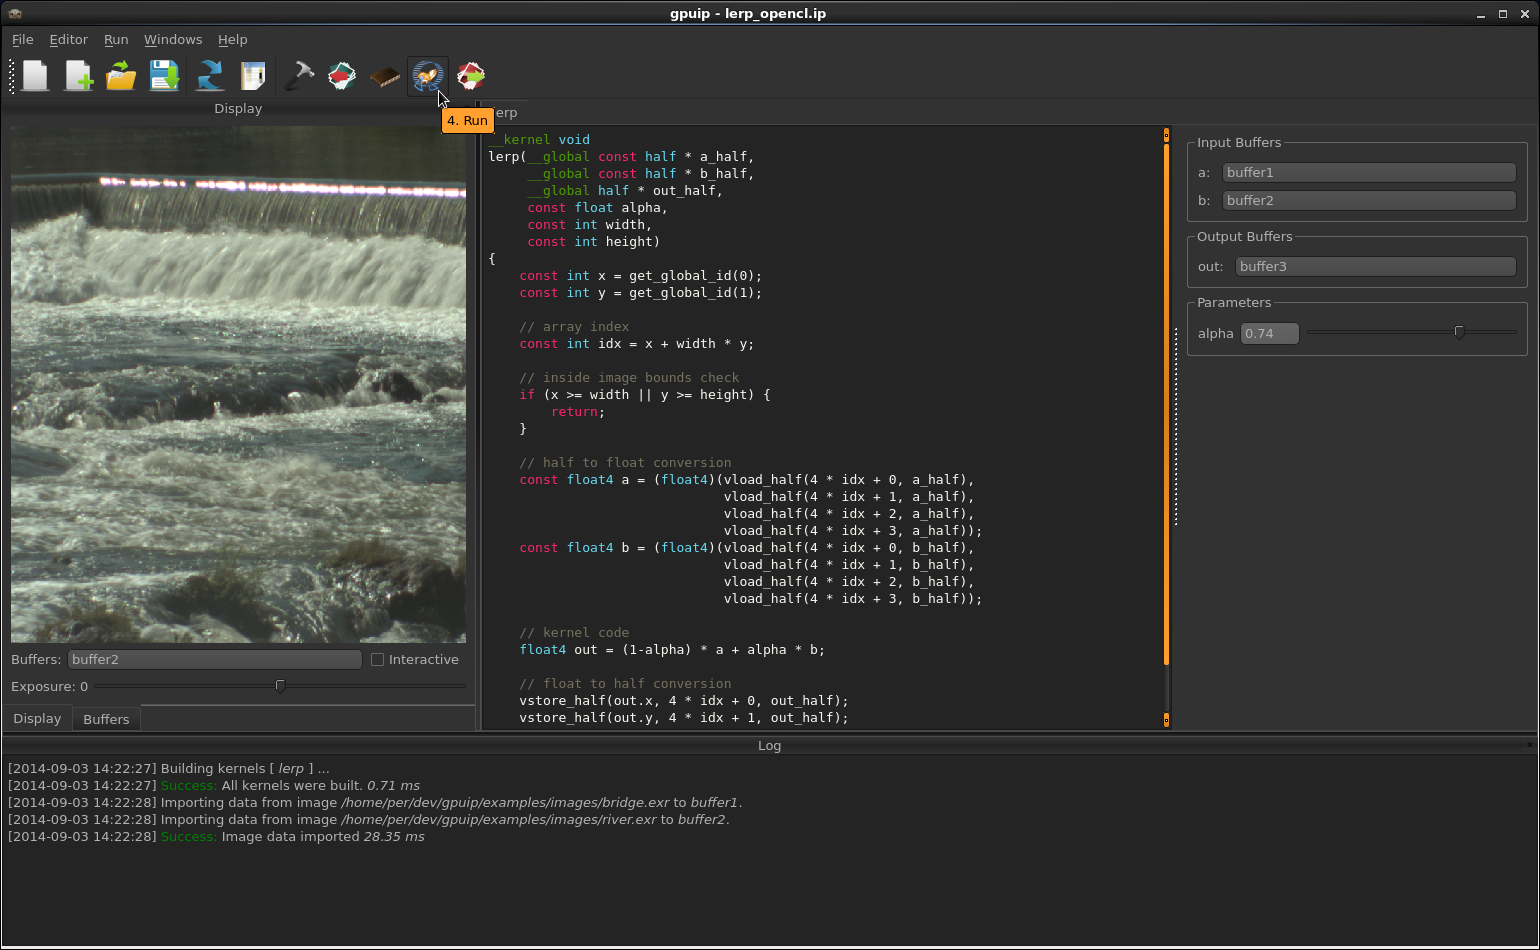
\includegraphics[width=140mm]{img/gpuip.png}
\caption{The gpuip GUI application.}
\label{gpuipgui}
\end{figure}
\end{center}

\begin{center}
\begin{figure}[!tbp]
  \centering
  \begin{minipage}[b]{0.4\textwidth}
    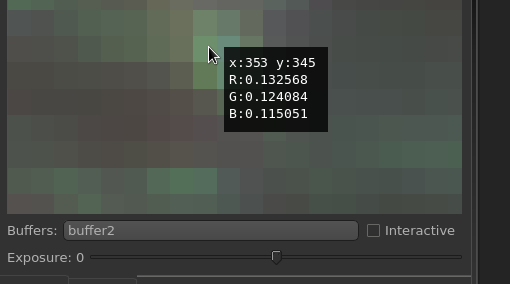
\includegraphics[width=60mm]{img/preview.png}
    \caption{Debug info pops up by right-clicking on the image in the Display view.}
  \end{minipage}
  \hfill
  \begin{minipage}[b]{0.4\textwidth}
    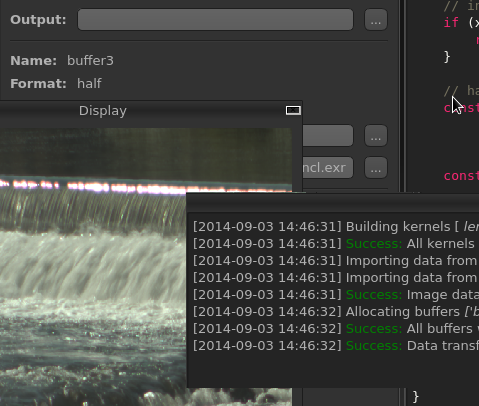
\includegraphics[width=60mm]{img/detach.png}
    \caption{All widgets can be detached.}
  \end{minipage}
\end{figure}
\end{center}

\begin{figure}[ht!]
\centering
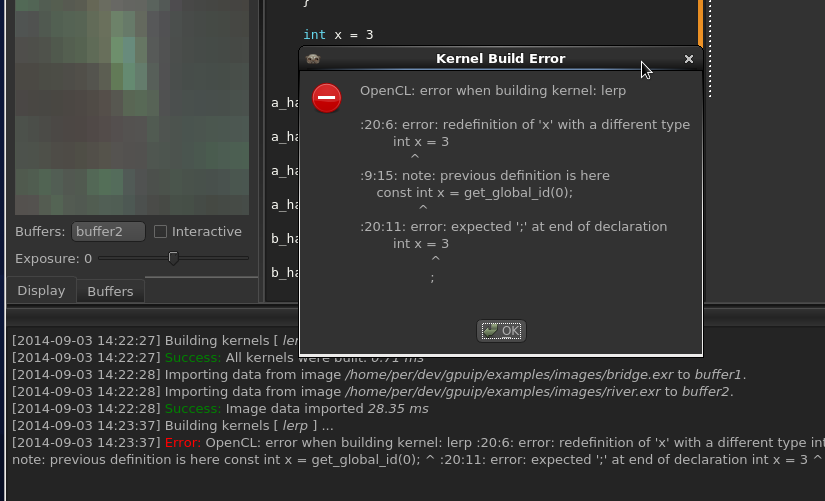
\includegraphics[width=80mm]{img/error.png}
\caption{Example of error feedback when compiling.}
\label{gpuippreview}
\end{figure}

\begin{figure}[ht!]
\centering
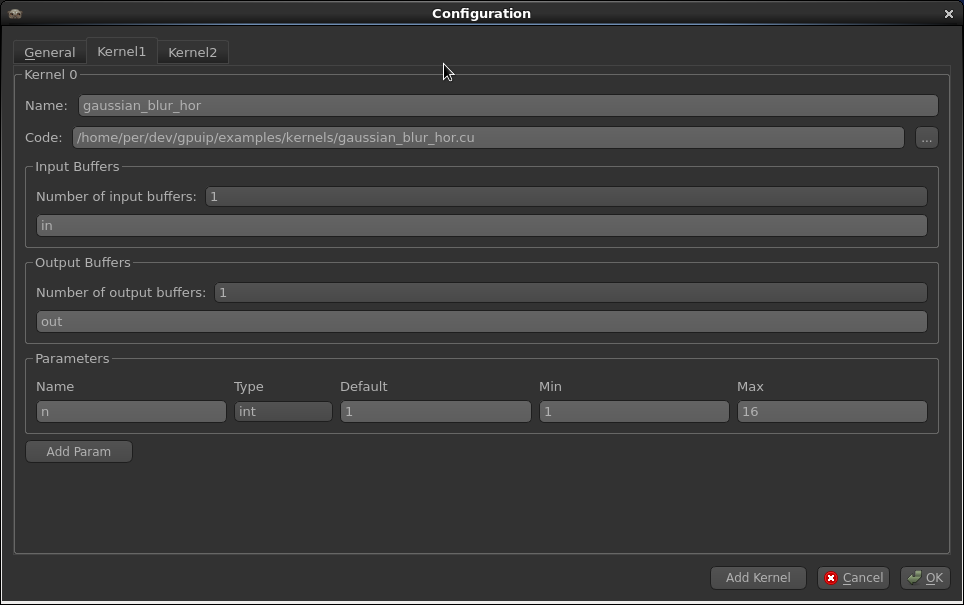
\includegraphics[width=80mm]{img/config.png}
\caption{Example of the configuration step when creating a new {\tt .ip} file.}
\label{gpuipconfig}
\end{figure}




